\section{Robot Players}
\label{sec:robot_players}
A match is played by two teams, each consisting of not more than \textbf{5} players. At most one player may be designated as \emph{goalkeeper}, the others are all \emph{field players}.

\subsection{Hardware}
\label{sec:hardware}
All teams must use black, gray, red, blue, or orange plated NAO humanoid robots manufactured by SoftBank Robotics.

Absolutely no modifications or additions to the robot hardware are allowed. No additional hardware is permitted including off-board sensing or processing systems. Additional sensors besides those originally installed on the robots are likewise not allowed. The only exceptions are:

\begin{itemize}
    \item Setting the passive wrist joints to a fixed position either with glue or a transparent or white duct tape.
    \item Protecting the fingers with white finger protectors provided by the manufacturer or with transparent or white duct tape.
    \item Placing white duct tape over the battery case and screw (under the robot jersey) to keep the battery case in place and prevent the battery becoming disconnected.
    \item A memory stick may remain in the head during operation.  Only ordinary USB flash memory keys that sit flush or recessed to the head casing may be utilized. Other USB dongles or devices, as well as memory sticks that are not flush or recessed, are not permitted.
\end{itemize}

A computer with two monitors (one for GC and one for TCM) will be provided by the event organizers for the purpose of sending GameController messages to the robots and observing if no robot violates the rules for WIFI usage.
Additionally, there should be at least one monitor mirroring the second screen of the GC PC with the TCM in visitor mode. \todo{Clearfy this, which TCM mode}

\subsection{Goal Keeper}
\label{sec:goal_keeper}

The goal keeper is allowed to touch the ball with its arms/hands only while it is within its own goal box area. It always has the jersey number ``1''.

\subsection{Field Players}
\label{sec:field_players}
Each of the four field players has a jersey number from the set $\{2, 3, 4, 5, 6\}$. However, by default, the number ``6'' should only be used for a substitute that enters the game later.

\subsection{Team Markers}
\label{sec:team_markers}

Robots use colored jersey shirts as team markers. Each jersey shirt has a player number (1-6) printed on it.  The team markers are worn as shown in Figure~\ref{fig:nao_markers}.

\begin{figure}
  \centerline{\begin{tabular}{lll}
      a) & b) & c) \\
      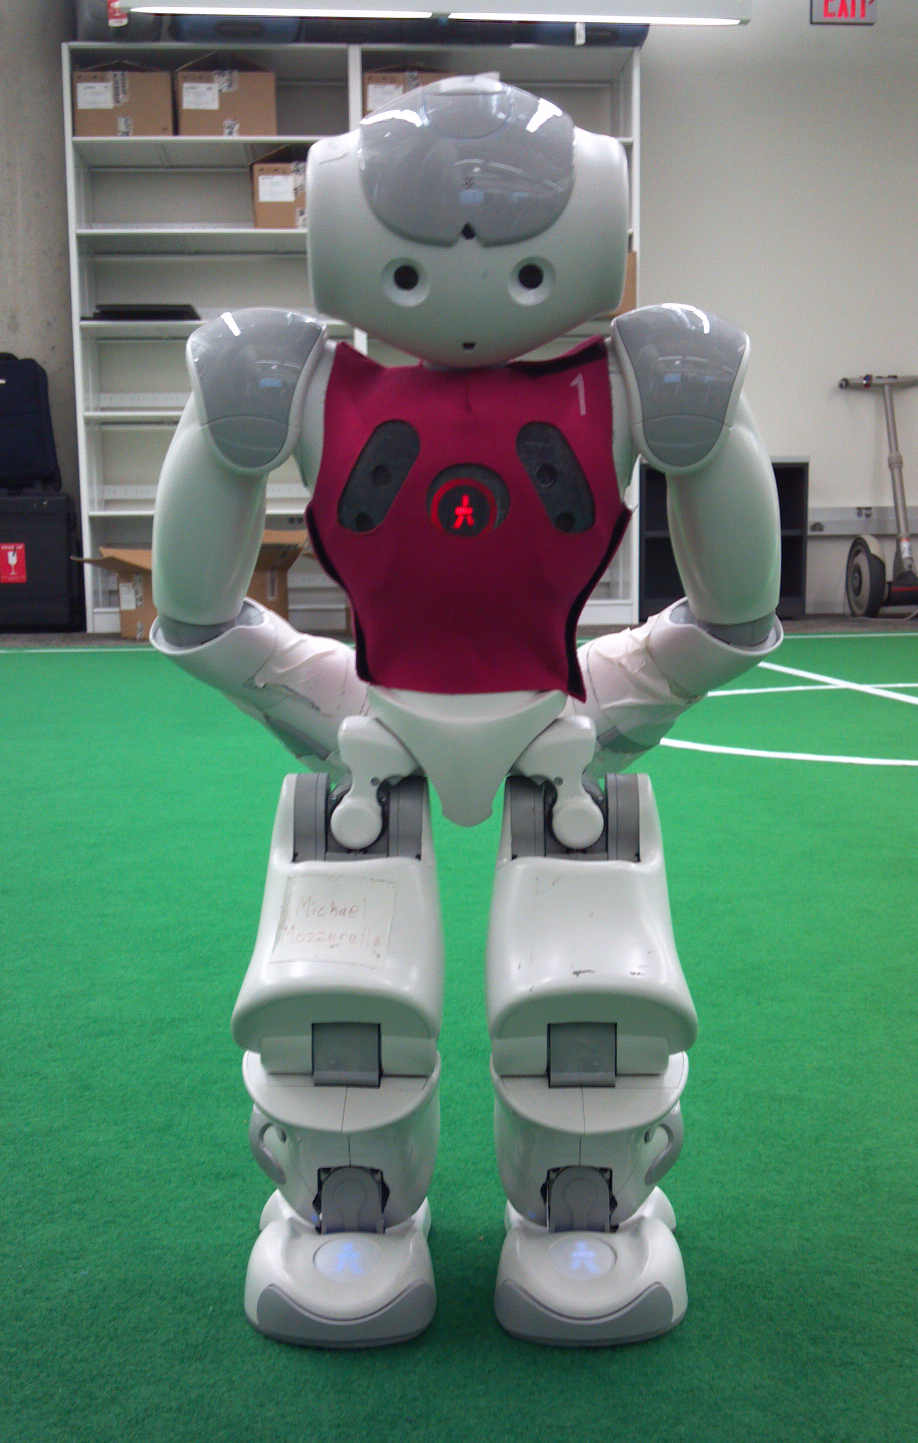
\includegraphics[height=0.28\columnwidth]{figs/front.jpg}&
      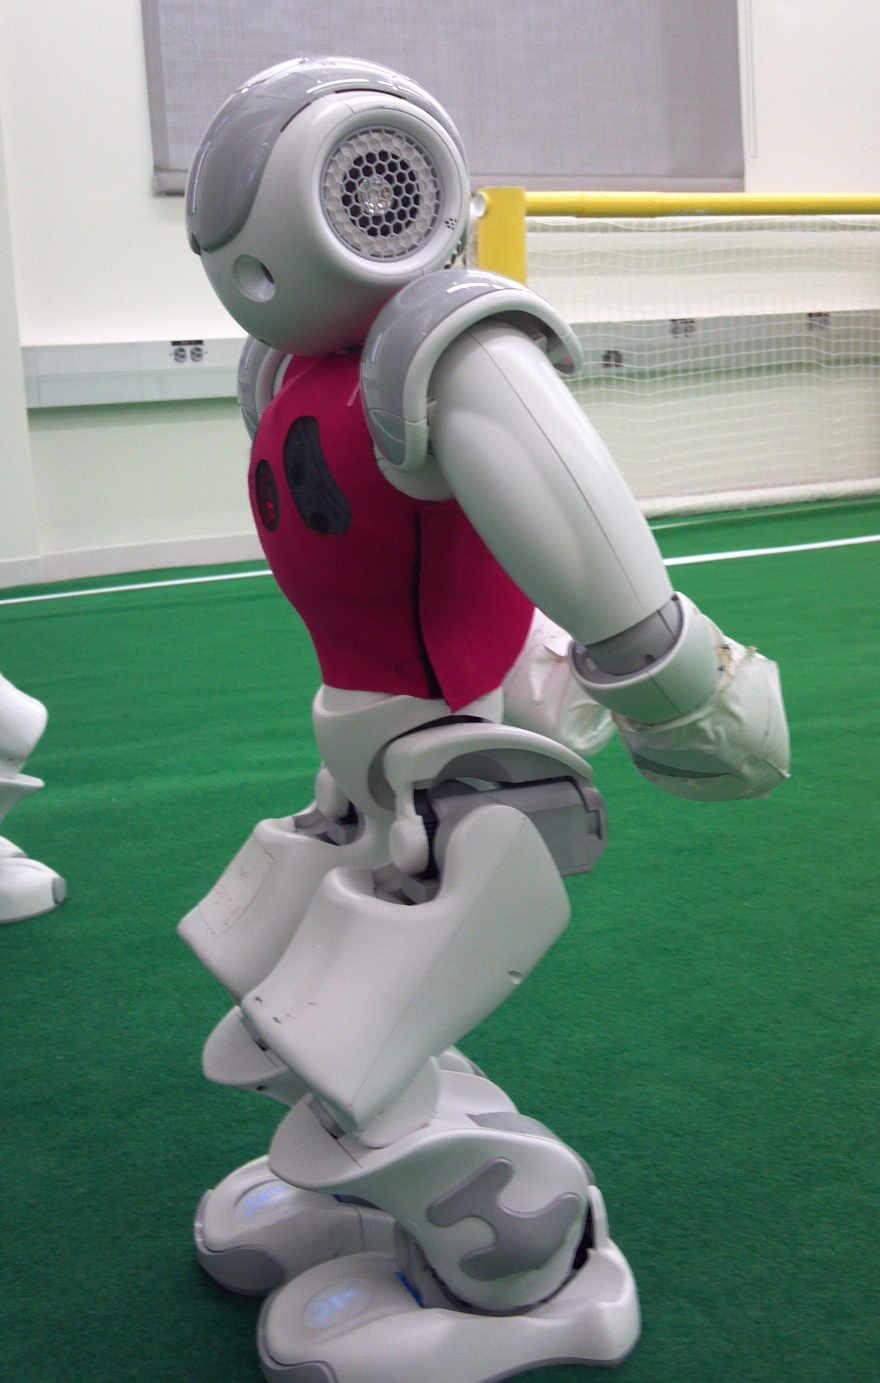
\includegraphics[height=0.28\columnwidth]{figs/side.jpg} &
      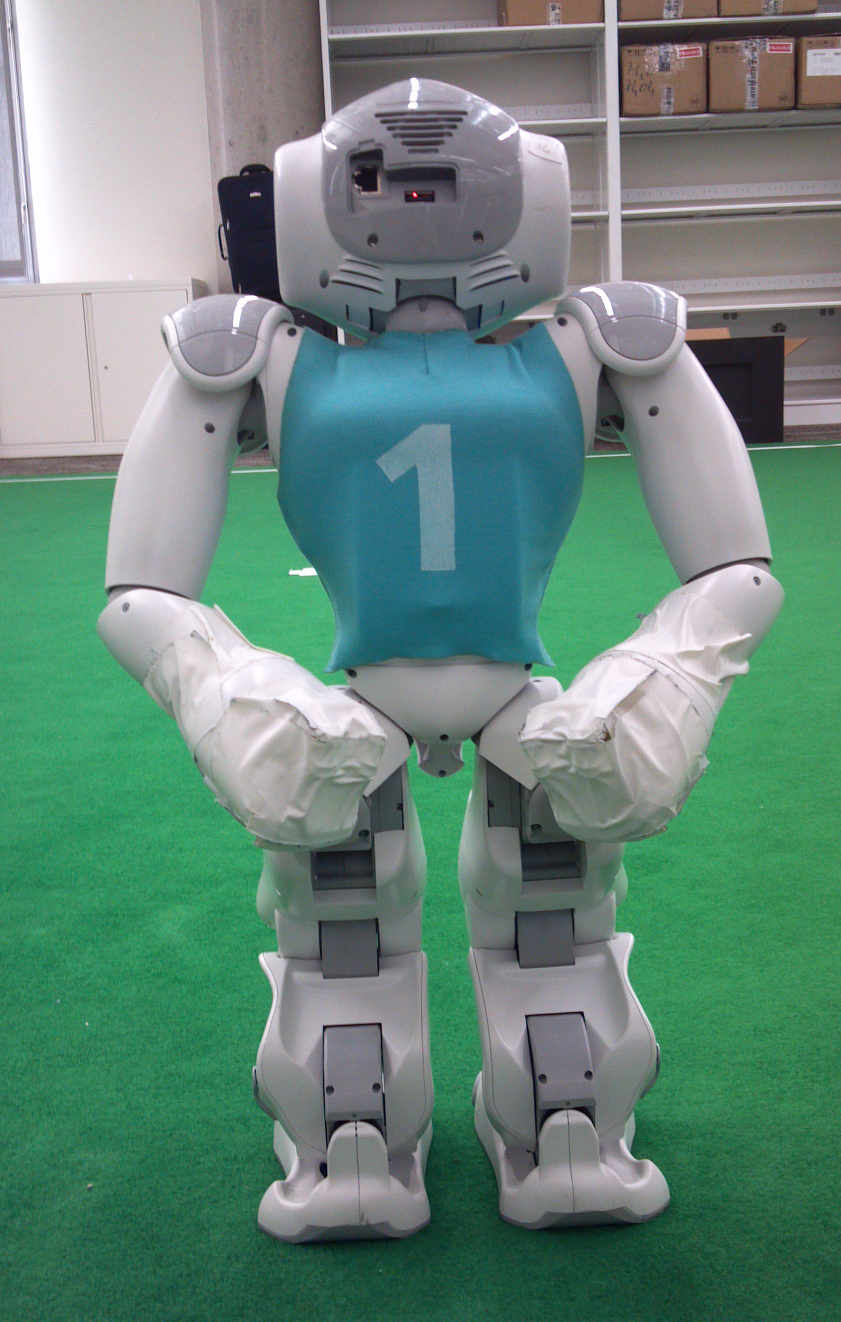
\includegraphics[height=0.28\columnwidth]{figs/back.jpg}
  \end{tabular} }
  \caption{Team markers. a) Front view. b) Side view. c) Back view.}
  \label{fig:nao_markers}
\end{figure}
Teams may use any jersey that was approved for a RoboCup SPL competition in the last 4 years without needing to reapprove it in 2022.\todo{Make parameter}

Teams may design and manufacture their own jerseys in any color (multi and many color jerseys are acceptable), but must follow these guidelines:
\begin{itemize}
\item Jerseys should be the \textbf{tank top} style used at RoboCup 2013/2014 and should cover approximately the same areas of the robot as shown in Figure~\ref{fig:nao_markers}. The torso LED must be clearly visible. Jerseys may include the sonar panel used in the 2013/2014 jerseys, although this is not required. Jerseys may not cover the shoulders of the robots.
\item Jerseys must have a primary color that comprises at least \qty{70}{\percent} of the jersey.
\item Jerseys should not contain distractors, such as large pictures of SPL balls or white stripes on green jerseys.
\item All players on a team must wear identical jerseys, including the goalkeeper.
\item A team must wear the jerseys that it starts a game in for the entire game.
\item Jersey material must be non-reflecting, non-shiny, and non-textured.  Material that is glittery is also not appropriate.
\item Jerseys should be numbered 1-6 on both sides.  The numbers must be large and {\bf easily} recognized by humans.
\item Teams must have two sets of jerseys that are significantly different in terms of their primary color.
\item Designs must be submitted to \url{rc-spl-tc@lists.robocup.org} for approval by \DTMdate{2022-05-01}.\todo{Make parameter} If the team has jersey prototypes, they should submit close-up images of a robot wearing the jersey — these images should be taken from front, back, and side angles.  If the team has no prototypes, then designs depicting the expected jersey should be submitted.  If submissions show separated front and back halves of jerseys then the team must specify which halves are matched to form home and away jerseys.  All images and designs should be submitted in pdf or jpg format.
\end{itemize}

Each team must designate a ``home'' color and an ``away'' color when asked about one month before RoboCup. Teams must wear their `home' jerseys when they are ```home'' (the first team listed on the schedule). Teams will wear their ``home'' jersey when they are ``away'' (the second team listed on the schedule) as well, unless either the head referee or the GameController program believes the jerseys of two competing teams are too similar.  In this case, the ``away'' team will then wear their ``away'' jersey.

Some teams wish to include additional information or logos on their robots. The following are allowable:

\begin{itemize}
  \item Attaching player numbers to the heads and/or legs of the robots. These numbers should be black with a white background, and should correspond to the number on the robot's jersey.

  \item Adding sponsor or team logos to the upper legs of the robots (\cf Figure~\ref{fig:sponsor}). A box drawn around the non-white area of these logos must not cover more than a \qty{25}{\square\centi\metre} area. At most one logo may be attached per leg - if you wish to attach more than one logo per leg, email the Technical Committee at least two weeks before the competition. Depending on the size and design of the logos, this may be allowable.

  \item Adding small black and white stickers to the torso of the robots stating the name of the robot, the name of the team, or similar information. These stickers must be small and mostly white.
\end{itemize}

\begin{figure}[b]
  \centerline{\begin{tabular}{ll}
  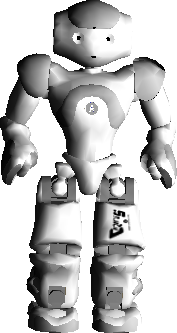
\includegraphics[height=0.35\columnwidth]{figs/naosim_with_logo.png}&
  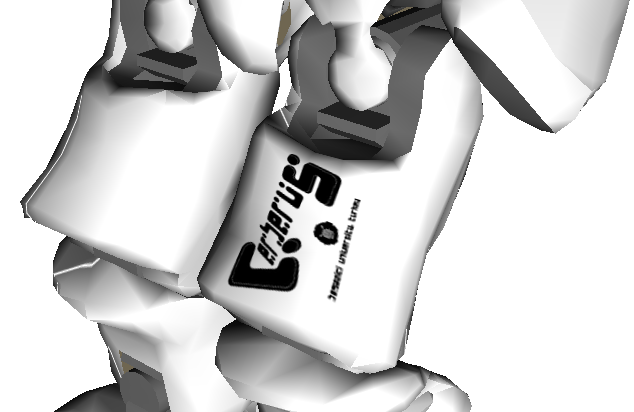
\includegraphics[height=0.35\columnwidth]{figs/naosim_legs_with_logo_closeup.png}
  \end{tabular}}
  \caption{Example Sponsor/Team Logo placement on legs.}
  \label{fig:sponsor}
\end{figure}

\subsection{Communications}

The robots must play without human control. Communication is only allowed among robots on the field and between the robots and the GameController.

\subsubsection{Non-Wireless Communications}
\label{sec:acoustic}
In general there are no restrictions on communication between robots in play on the field using visual signalling (\eg gestures) or the robot's built-in microphones, speakers, and infrared transceivers. However, communication that causes excessive discomfort to an audience, affects the safety of an audience, or violates normal playing rules is not permitted.

\subsubsection{Wireless Communications}
\label{sec:wireless}
The only wireless hardware allowed to be used by the teams are the wireless network cards built into the NAOs, and the access points provided by the event organizers. All other wireless hardware must be deactivated. A team may be disqualified if one of the team members violates this rule.

Each team will get a range of IP addresses that can be used both for their robots and their computers. The network configuration (\eg IP addresses, channels, SSIDs, and required encryption) of the fields will be announced at the competition site.

Wireless robot-to-robot communication among the robot players is allowed, as long as it uses the access points provided by the event organizers (using the so-called ad-hoc mode is prohibited), messages are sent via UDP broadcast, and the SPL standard message packet is used. The SPL standard message packet is specified in the header \emph{SPLStandardMessage.h} that is distributed with the latest GameController release at \url{https://github.com/RoboCup-SPL/GameController}.

Each team will be assigned a range of IP-addresses that can be used for robot-to-robot communication. Each team will also be allocated a single UDP port for network broadcasts. Specifically, a team's port will be 10000 plus that team's GameController number. All robot-to-robot communication during matches must be sent via UDP broadcast. Unicast communication between robots is prohibited.

The amount of data transmitted by a team in a single game is limited. The limit is measured as the total number of UDP packets sent by any robots of a team. A team may not exceed \TeamMessageLimit packets per game. This limit will be lowered in future competitions to encourage smart event-based communication. If a team exceeds their limit the game is scored with 0 goals for the offending team. Robot-to-robot communication that violates the SPL rules result in a game scored with 0 goals for the offending team (even when discovered after the game was finished).

The GameController tracks the number of messages that have already been sent and includes the counters per team in \texttt{RoboCupGameControlData}.

In addition to robot-to-robot communication, robots may send:
\begin{itemize}
 \item Additional status update packages that are sent to the GameController.
 \item Team specific debug information may be sent to an external computer owned by the team. A robot may send debug information at most once every 2 seconds in a single UDP packet.
\end{itemize}
These additional packages do not count towards the team's data limit and may not be used for robot-to-robot communication. They must be sent as unicast and may not be sent as broadcast.

Teams and their robots must not listen into another team's communication.

Robots are not allowed to be connected to access points of fields that are currently running official games of other teams.
Robots may only communicate on fields that are not running an official game or fields which they are playing on.

The GameController will use UDP to connect to the robots. The source distribution of the GameController provides the header file \emph{RoboCupGameControlData.h} that defines all messages sent by the GameController to the robots. They correspond to the \emph{robot states} described in Section~\ref{sec:robot_states}.

Robots send status updates (defined in \emph{RoboCupGameControlData.h}) to the GameController. These return packets must be addressed directly to the GameController PC (\ie not broadcast) and sent on the GameController return UDP port specified by the symbol \verb!GAMECONTROLLER_RETURN_PORT! in \emph{RoboCupGameControlData.h}.

The use of remote processing/sensing is prohibited.
